%%% ----- general packages and settings ----- %%%
\documentclass[a4paper, ngerman, bibliography=totoc]{scrreprt}  %%, listof=totoc
\usepackage[T1]{fontenc}
\usepackage[utf8]{inputenc}
\usepackage{lmodern}
\usepackage{babel}
\usepackage{microtype} % fixes line breaks

%%% ----- bibliography ----- %%%
\usepackage[babel, german=quotes]{csquotes}
\usepackage[backend=biber, style=alphabetic-verb]{biblatex}
\bibliography{literatur}
\DeclareFieldFormat[article]{title}{#1\isdot} % http://golatex.de/formatierung-des-literaturverzeichnisses-mit-biblatex-t3988.html

%%% ----- references (http://tex.stackexchange.com/a/83051) ----- %%%
\usepackage{varioref}
\usepackage[breaklinks]{hyperref}
\usepackage{cleveref}
\crefname{lstlisting}{Quelltext}{Quelltext}

%%% ----- listings ----- %%%
\usepackage{xcolor} % http://tex.stackexchange.com/a/150377
\usepackage{listings}
\renewcommand{\lstlistingname}{Quelltext}
\renewcommand*{\lstlistlistingname}{Quelltextverzeichnis}

\definecolor{strings}{rgb}{0.69, 0.196, 0.267}
\definecolor{comments}{rgb}{0.247, 0.518, 0.173}
\definecolor{keywords}{rgb}{0.114, 0.180, 0.992}
\definecolor{linenumbers}{rgb}{0.25, 0.25, 0.25}
\definecolor{linebreakmarker}{rgb}{0.25, 0.25, 0.25}

\lstset{ %
  belowcaptionskip=1\baselineskip{},
  breaklines=true,
  postbreak=\mbox{\textcolor{linebreakmarker}{$\hookrightarrow$}\space},
  captionpos=b,
  commentstyle=\color{comments},
  keywordstyle=\color{keywords}\bfseries,
  morecomment=[s][\color{comments}]{/**}{*/},
  numbers=left,
  numbersep=16pt,
  numberstyle=\tiny\color{linenumbers},
  stringstyle=\color{strings},
  tabsize=2
}

%%% ----- graphics ----- %%%
\usepackage{graphicx}

%%% ----- fix underscore problems ----- %%%
\usepackage[strings]{underscore}

%%% ----- prevent word breaks ----- %%%
\hyphenation{ECMAScript}

%%% ----- custom commands ----- %%%
% - circled numbers (http://tex.stackexchange.com/a/7045)
\usepackage{tikz}
\newcommand*\circled[1]{\tikz[baseline=(char.base)]{\node[shape=circle,draw,inner sep=2pt] (char) {#1};}}
% - z.B. (http://latex.hpfsc.de/content/latex_tipps_und_tricks/eigene_kommandos/)
\newcommand{\zB}{z.\,B. }


%%% ---------- Document Data ----------
\title{softaware/webdev-Container}
\subtitle{Ein Docker-Container zur konsistenten Entwicklung\\von JavaScript-basierten Webprojekten}
\author{Bernhard Mayr}
\date{\today}

\begin{document}
\maketitle
\setcounter{page}{58}
\addchap{Kurzfassung}
Softwareentwicklung in Zeiten von Node.js, ASP.NET Core und Microservices impliziert die Verwendung einer Menge an Werkzeugen.
Die Hauptaufgabe des Softwareentwicklers ist es allerdings, Software zu entwickeln und nicht den Großteil seiner Zeit mit dem Erlernen und der Konfiguration dieser Werkzeuge zu verbringen.

Mit Docker wurde eine Plattform zur Vereinfachung der Softwareentwicklung auf Basis von Containervirtualisierung geschaffen, deren Ziele eine möglichst einfache Verwendung und Plattformunabhängigkeit sind.
Anhand der Geschichte der Containervirtualisierung wird in dieser Arbeit ein Vergleich zu herkömmlichen Virtualisierungsmöglichkeiten gezogen sowie die Funktionsweise und notwendigen Systemvoraussetzungen für die Verwendung von Containern dargestellt.
Nach einer Übersicht über bestehende Werkzeuge des Konfigurationsmanagements wird für Softwareentwickler eine Einführung in die Verwendung von Docker zu Entwicklungszwecken gegeben, wobei besonders auf Best-Practices und Integrationsmöglichkeiten in den Entwicklungsprozess Wert gelegt wird.

Am Beispiel verschiedener Anwendungsfälle wird gezeigt, wie der Entwicklungsprozess mithilfe von Docker stabiler und einheitlicher gestaltet werden kann, um das erklärte Ziel, einen produktiveren und angenehmeren Workflow für Softwareentwickler, zu erreichen.

Aktuelle Entwicklungen wie Eclipse Che und Windows Container zeigen, dass Containervirtualisierung im Allgemeinen und Docker im Speziellen eine große Zukunft bevorsteht.

\addchap{Abstract}

\tableofcontents
\chapter{Einleitung}
\section{Motivation}
Die tägliche Arbeit eines Softwareentwicklers beinhaltet die Verwendung von zahlreichen Werkzeugen.
Besonders bei der Entwicklung auf unterschiedlichen Plattformen führt die Kombination der zahlreichen Build-Tools, Compiler, Transpiler, Task-Runner, Paketmanager und Datenbanken schnell zu einer umfangreichen Kombination an Kommandos.
Projekte entwickeln sich weiter und neue Technologien erscheinen, schnell wird aus einem \texttt{npm run dev} ein \texttt{npm start} oder \texttt{mvn build} bricht aufgrund einer falschen Java-Version ab.
Die große Vielfalt der Werkzeuge, besonders im Web-Bereich, verlangt vom Entwickler, dass er sich für jedes Projekt das Wissen für ein neues Werkzeugset aneignet und dieses auch zu verwenden weiß.

Seit 2014 verspricht Docker mit dem Werbespruch \emph{"`Build, Ship, Run"'} eine Verbesserung des Softwareentwicklungsprozesses mithilfe von Containervirtualisierung.
Welche Möglichkeiten der Automatisierung für den Softwareentwickler gegeben sind, inwieweit ein plattformunabhängiger Entwicklungsprozess möglich ist und ob sich durch den Einsatz von Docker die Lernkurve eines Entwicklers beim Einstieg in ein Softwareprojekt verringern lässt, sind motivierende Gründe für diese Bachelorarbeit.

\section{Ziel}
Durch exemplarisches Lösen typischer Probleme, mit denen Softwareentwickler häufig konfrontiert sind, soll dem Leser die Verwendung und Flexibilität von Docker gezeigt werden.
Weiters sollen Softwareentwickler automatisierbare Probleme erkennen und verstehen, ob und wie Docker in diesen Fällen zu einer zeit- und ressourcensparenden Lösung beitragen könnte.

Zur Verdeutlichung dieser entwicklergesteuerten Sicht auf Docker werden in der Arbeit verschiedene Virtualisierungstechniken verglichen und in der Funktionsweise und dem Einsatzzweck von Docker abgegrenzt.
Die grundlegenden, für den Entwickler notwendigen Konzepte von Docker werden ebenso geschildert wie eine Übersicht und Erklärung der in Verbindung mit Docker am häufigsten eingesetzten Werkzeuge.

% \section{Glossar}
% \begin{description}
%    \item[Vollvirtualisierung]
%    \item [DevOps]
% \end{description}

\chapter{Aktuelle Probleme der Frontend-Webentwicklung}
\label{cha:frontend-problems}

Das größte Problem der Frontend-Webentwicklung wird in \autocite{Kirejczyk.HDD:online} \emph{Hype Driven Development} genannt.
Damit ist die enorm hohe Frequenz gemeint, in der neue Technologien entstehen, hochgepriesen werden und danach genau so schnell wieder von neueren abgelöst und verdrängt werden.

Gerade im Web-Bereich ist durch den Trend zu Open Source Software eine sehr hohe Obsoleszenz zu beobachten, da durch das abzweigen (engl. \emph{forken}) verschiedene Varianten von gesamten Projekten entstehen.
Dem dadurch entstehenden schnellen Fortschritt steht allerdings die Spaltung von Entwicklergemeinschaften und inkompatible Technologien gegenüber.

Ein Beispiel dafür ist die Teilung von Node.js\footnote{\url{https://nodejs.org/}} in die zwei Projekte Node.js und io.js\footnote{\url{https://iojs.org/}} im Jahr 2014, die allerdings aus den vorhin beschriebenen Problemen 2015 wieder zu Node.js vereint wurden \autocite{Node.io-node-merge:online}.
Kurzlebige, innovative Technologien bringen die Softwareentwicklung im Generellen voran, doch um eine Technologie in seriösen Anwendungen verwenden zu können, ist ein gewisser Reifegrad notwendig.
Dieser ermöglicht nicht nur stabile Versionen und besser ausgebildete Entwickler, durch einen Einzug der Technologie in die Lehre, sondern vor allem durchdachte und ausgereifte Werkzeuge für Entwickler.

Nach erfolgreicher Auswahl eines Frameworks ist in der Frontend-Entwicklung die größte Hürde die Konfiguration der benötigten Werkzeuge.
Die Schwierigkeit liegt wiederum in der beinahe täglichen Aktualisierung der Werkzeuge, die teilweise inkompatible Änderungen verursachen und dem ständigen Erscheinen neuer Werkzeuge.
Hilfsanwendungen wie create-react-app\footnote{\url{https://github.com/facebookincubator/create-react-app}} oder Angular CLI\footnote{\url{https://github.com/angular/angular-cli}} erleichtern die Erstellung von Webanwendungen, indem sie ein initiales Projekt konfigurieren, in dem bereits alle benötigten Abhängigkeiten und Werkzeuge integriert sind.

Im Folgenden werden einige der Werkzeuge beschrieben, um einerseits deren Schnellebigkeit zu veranschaulichen und andererseits einen Überblick zu liefern, welche Werkzeuge wozu aktuell eingesetzt werden.

\section{Werkzeugübersicht}
\label{sec:tools-overview}

\subsection{JavaScript-Modulsysteme}
\label{sub:js-modulesystems}
% https://auth0.com/blog/javascript-module-systems-showdown/
\subsubsection{CommonJS}
\label{sub:commonjs}
\subsubsection{AMD}
\label{sub:amd}
\subsubsection{ES2015}
\label{sub:es2015}


\subsection{Paketmanager}
\label{sub:package-managers}

Lokale vs. Globale Installation
Angular CLI

% http://andrewhfarmer.com/javascript-frontend-package-managers/

\subsubsection{npm}
\label{sub:npm}
\subsubsection{bower}
\label{sub:bower}
% https://gofore.com/stop-using-bower/
% https://shellmonger.com/2015/07/26/moving-from-bower-to-npm/
% https://www.quora.com/Why-use-Bower-when-there-is-npm
% https://stackoverflow.com/questions/18641899/what-is-the-difference-between-bower-and-npm
\subsubsection{yarn}
\label{sub:yarn}
\subsubsection{jspm}
\label{sub:jspm}
\subsubsection{Duo}
\label{sub:duo}



\subsection{Build-Werkzeuge}
\label{sub:build-tools}

% http://ericlathrop.com/2017/05/the-problem-with-npm-install-global/

\subsubsection{grunt}
\label{sub:grunt}
\subsubsection{gulp}
\label{sub:gulp}
\subsubsection{webpack}
\label{sub:webpack}
\subsubsection{rollup}
\label{sub:rollup}
% https://medium.com/webpack/webpack-and-rollup-the-same-but-different-a41ad427058c
\subsubsection{Best Practice}
\label{sub:build-tools-best-practices}


\section{Inkompatible node/npm-Versionen}
Die Basis für die meisten Werkzeuge in der Frontend-Webentwicklung bildet \emph{Node.js}.
Node.js ist eine Laufzeitumgebung, die auf der Chrome-V8-JavaScipt-Engine basiert und es ermöglicht, JavaScript ohne Browser auf dem System nativ auszuführen.
Der große Vorteil, der vor allem Entwicklerwerkzeuge betrifft, ist die Plattformunabhängigkeit.
Dadurch können Kommandozeilenwerkzeuge mithilfe von Webtechnologien für alle gängigen Betriebssysteme erstellt werden.

\emph{npm} ist ein Paketmanager, der es ermöglicht Node.js-Anwendungen zu installieren, oder Abhängigkeiten zwischen Paketen zu spezifizieren.

Wie in \autocite{Papa.n:online} beschrieben, kann es nun allerdings sein, dass bestimmte Werkzeuge unter bestimmten Node.js-Versionen nicht funktionieren.
Auch das Testen von Anwendungen unter verschiedenen Node.js-Versionen gestaltet sich schwierig, da dafür jedesmal eine Neuinstallation notwendig ist.
Ein weiteres Problem ist, dass die benötigte Node.js-Version bei Projekten nicht mitversioniert werden kann.
Sie kann maximal in einer Readme-Datei erfasst werden, wobei jeder Entwickler selbst sicherstellen muss, dass er die korrekte Version verwendet.
Bei der Entwicklung mehrerer Projekte wird dieses Problem noch ersichtlicher.


\section{Parallele Entwicklung mehrerer Projekte}
Wie in \cref{sec:softaware} erläutert, ist es in der Firma softaware gmbh üblich, dass ein Entwickler an mehreren Projekten gleichzeitig arbeitet.
Dadurch tritt das vorhin erwähnte Problem häufiger auf, da es nun vorkommen kann, dass bei der Entwicklung unterschiedlicher Projekte unterschiedliche Node.js-Versionen notwendig sind.

Ein Lösungsansatz dafür ist die Verwendung von Vagrant\footnote{\url{https://www.vagrantup.com/}}. 
Vagrant ist ein Werkzeug zur automatischen Verwaltung von virtuellen Maschinen und ermöglicht dadurch die deklarative Beschreibung von Entwicklerrechnern.
Diese Beschreibung kann mitversioniert werden, wodurch eine konsistente Arbeitsumgebung entsteht.
Eine virtuelle Maschine benötigt allerdings erhebliche Ressourcen, wodurch es, wenn keine grafische Oberfläche benötigt wird, bessere Lösungsansätze gibt.

Ein weiterer Ansatz ist die Verwendung von sogenannten Node.js-Versionsmanagern.
Beispiele dafür sind nvm\footnote{\url{https://github.com/creationix/nvm}}, n\footnote{\url{https://github.com/tj/n}} oder nvm-windows\footnote{\url{https://github.com/coreybutler/nvm-windows}}.
Das Hauptproblem dabei ist allerdings, dass es keine Lösung gibt, die plattformübergreifend funktioniert.
Außerdem wurde die Entwicklung des als letztes erwähnten nvm-windows eingestellt, wodurch für Windows keine aktuelle Lösung existiert.
Ein weiteres Problem ist die fehlende Integration in den Quelltext des Softwareprojektes.
Daher werden diese Werkzeuge als eigenständige Anwendung auf dem Entwicklerrechner installiert und stellen lediglich eine implizite Abhängigkeit des Projektes dar, die nur schwierig automatisch installiert werden kann.

Nicht nur die parallele Entwicklung mehrerer Projekte kann Probleme bereiten.
In der Firma softaware gmbh kommt es außerdem regelmäßig vor, dass andere Unternehmen als Projektpartner fungieren.
Gerade in diesem Fall ist es wichtig, eine einheitliche Lösung zur Verwaltung von Node.js-Versionen zu finden, da für diese Projektpartner die Hemmschwelle zur gemeinsamen Entwicklung möglichst niedrig sein soll.


\section{Globale Installation von npm-Paketen}
Bei der vorhin erwähnten Installation von npm-Paketen existieren zwei Möglichkeiten.

Für diverse Werkzeuge wird als Installationskommando \verb|npm install -g <Werkzeug>| vorgeschlagen, wobei das Paket durch den Parameter \verb|-p| global installiert wird.
Diese Art der Installation bedeutet, dass diese Anwendungen mit ihrem jeweiligen Namen direkt von der Kommandozeile gestartet werden können.
Diese Funktionalität hört sich sehr verlockend an, erfordert allerdings, dass jeder Entwickler dieses Werkzeug global installiert.
Dies mag in einer Abteilung problemlos funktionieren, wird aber spätestens bei Open-Source-Projekten zum Problem, da der Einstieg in ein Projekt dadurch erheblich komplizierter wird.
Außerdem kann es zu Versionsproblemen kommen, falls zwei Projekte dasselbe Werkzeug in unterschiedlichen Versionen benötigen, da global lediglich eine Version installiert werden kann.

Die zweite Möglichkeit der Installation ist das Weglassen des Parameters \verb|-p|, wodurch das Paket in der Manifest-Datei \verb|package.json| des Projekts erfasst und in einen Ordner namens \verb|node_modules| im aktuellen Verzeichnis installiert wird.
Da dieses Paket nun als Abhängigkeit erfasst ist, lässt es sich mit dem Projekt gemeinsam versionieren und wird bei der Installation dessen auf einem anderen Entwicklergerät automatisch mitinstalliert.
Allerdings lassen sich diese Pakete nun nicht mehr mit ihrem Namen auf der Kommandozeile ausführen, weshalb es verlockend klingen mag, \verb|./node_modules/.bin/| zur \verb|$PATH|-Variable hinzuzufügen.
Dadurch können lokal installierte Pakete einfacher ausgeführt werden, doch diese Änderung birgt zwei wesentliche Probleme.
Erstens müsste dies jeder Entwickler machen, wodurch eine einfache Zusammenarbeit erschwert wird und wieder eine implizite Abhängigkeit des Projektes entsteht.
Das wesentlich schwerwiegendere Problem betrifft allerdings die Sicherheit des Rechners.
Wie in \autocite{stackoverflow:nodemodules-hack:online} beschrieben, ermöglicht es diese Änderung der Systemvariable Angreifern infizierte Versionen von Standardprogrammen wie \verb|ls| oder \verb|cd| unter \verb|./node_modules/.bin/| abzulegen und dadurch kompletten Zugriff auf das Gerät zu erlangen.

\subsubsection{Empfohlene Vorgehensweise}
Um die Vorteile von global und lokal installierten Paketen zu kombinieren, gibt es bei dem Installieren von npm-Paketen den Parameter \verb|--save-dev|.
In der Manifestdatei \verb|package.json| existiert ein eigener Bereich \emph{devDependencies} in dem Werkzeuge erfasst werden, die für das Projekt benötigt werden.
Zusätzlich bietet das Manifest mithilfe der \emph{npm-scripts} die Möglichkeit eigene Namen für Kommandos zu vergeben, die dann mit \verb|npm run <Skriptname>| gestartet werden können.
Der Ausführungskontext dieser Kommandos beinhaltet automatisch den Pfad \verb|./node_modules/.bin/|, wodurch dort installierte Werkzeuge verwendet werden können.
Dies ermöglicht einheitliche Kommandos und eine automatische Dokumentation über Plattformgrenzen hinweg.

Außerdem bietet es den Vorteil, dass das intern verwendete Werkzeug ausgetauscht werden kann (\zB webpack anstatt gulp), für den Entwickler das Kommando aber weiterhin \verb|npm run build| bleibt und er durch diesen Austausch nichts Neues lernen muss.


\section{Legacy-Anwendungen}
\label{sec:legacy-applications}

\chapter{Lösungsvorschlag auf Basis von Docker}
\label{cha:possible-solution}

- Warum Container
- Versionierung/Commitable
- Abhängigkeiten
- CLI enough
- Auto-Install


Projektbasiertes Arbeiten + Partner bei softaware

\chapter{Erstellung des softaware/webdev-Docker-Containers}
\label{cha:implementation}
In diesem Abschnitt wird beschrieben, aus welchen Bestandteilen der Container besteht, warum diese Entscheidungen getroffen wurden und welche Probleme und Hürden sich bei der Entwicklung ergaben.
Weiters wird dargestellt, in welchen Aspekten der Container durch neue Kenntnisse beim Einsatz in echten Projekten weiterentwickelt wurde.

\section{Anwendungsszenarien}

run npm
add as dependency
inherit

\begin{lstlisting}[caption=Kommando zum Starten des softaware/webdev-Containers, language=bash, label=lst:docker-run-webdev]
docker run -it --rm -v ${pwd}:/usr/app/src softaware/webdev:alpine-8.1.2
\end{lstlisting}

\begin{figure}[htbp]
    \centering
    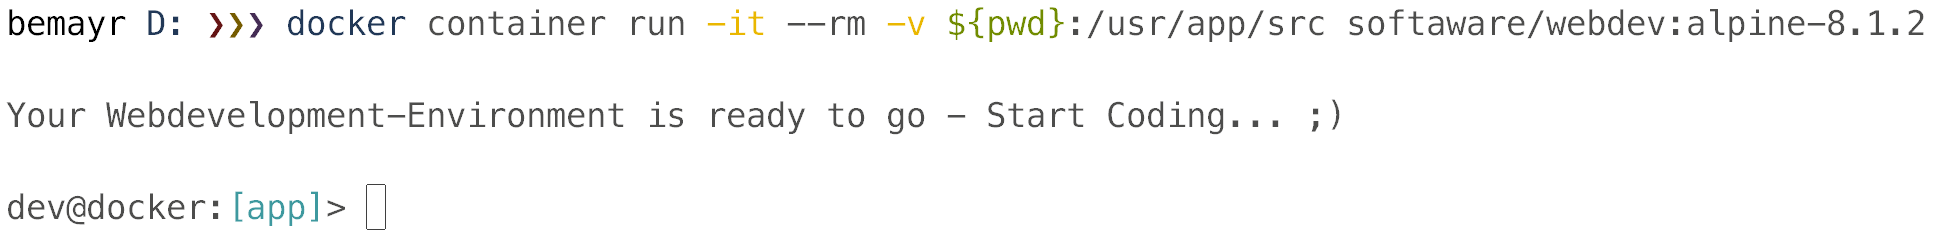
\includegraphics[width=0.92\linewidth,clip]{images/container-execution}
    \caption{Ausgabe beim Start des Containers}
\label{fig:container-execution}
\end{figure}

\section{Dockerfile}
\label{sec:dockerfile}
\lstinputlisting[caption=Alpine-Dockerfile,label={lst:dockerfile.alpine}]{listings/Dockerfile.alpine}

\lstinputlisting[caption=Bash-Konfigurationsdatei,label={lst:.bashrc},language=bash]{listings/.bashrc}

https://tex.stackexchange.com/questions/144170/lstlistings-reference-to-line-number
https://tex.stackexchange.com/questions/116216/is-there-a-possibility-to-make-reference-to-the-line-in-the-lstlisting-environme

Volumes
. Node modules Typescript
. Port mappings + Geschichte des Containers

https://docs.npmjs.com/cli/completion

run command
https://serverfault.com/questions/685697/multiple-commands-in-docker-cmd-directive
% https://docs.docker.com/engine/reference/builder/#cmd

\subsubsection{Zeile 2}
Die \verb|FROM|-Anweisung ermöglicht es Docker-Images voneinander zu erben.
In diesem Fall wird vom offiziellen node-Image\footnote{\url{https://hub.docker.com/_/node/}} geerbt.
Dieses beinhaltet Node.js, npm und yarn, wodurch die gesamte Basisfunktionalität bereits vorhanden ist.

\verb|{{ node_version }}| ist keine Funktionalität von Docker, dies ist ein Platzhalter für die Versionsnummer des Node.js-Images im Build-Prozess (vgl. \cref{sec:build-process}).
Der Name des offiziellen Node.js-Images beginnt mit der Node.js-Versionsnummer und enthält die Art des Images als Suffix.
In diesem Fall wird von dem \emph{alpine}-Image abgeleitet und der Platzhalter im Build-Prozess durch die konkrete Versionsnummer ersetzt.

\subsubsection{Zeile 3}
Die früher verwendete \verb|MAINTAINER|-Anweisung in Dockerfiles wurde durch das flexiblere \verb|LABEL| ersetzt.
Durch den \emph{maintainer} werden Metadaten erstellt, die angeben wer für dieses Image verantwortlich ist, und an wen sich der Benutzer dessen wenden kann.

\subsubsection{Zeile 6}
Wie im Kommentar in Zeile 5 beschrieben, wird durch die \verb|ENV|-Anweisung die Umgebungsvariable \verb|PATH| erweitert.
Diese Änderung ermöglicht es, lokal installierte Node.js-Anwendungen als Kommandos zu verwenden.

In \cref{sec:global-package-installation} wurde bereits der Unterschied zwischen global und lokal installierten Anwendungen erläutert.
Im Container ist allerdings aufgrund der Isolierung das in \autocite{stackoverflow:nodemodules-hack:online} beschriebene Sicherheitsrisiko wesentlich geringer.
Anstatt der Erstellung eines eigenen Container-Images mit global installierten Paketen, sollten diese bei der Verwendung des Containers immer in der \emph{package.json}-Datei erfasst werden.
Dadurch muss kein eigenes Image gewartet werden und auch ohne dem Container sind alle Abhängigkeiten des Webprojektes definiert.

Diese Änderung an der Umgebungsvariable ist lediglich aus Kompatibilitätsgründen vorhanden, damit auch ältere Projekte, die sich historisch bedingt auf globale Abhängigkeiten verlassen, im Container verwendet werden können.
Die Konfiguration eines Webprojektes sollte allerdings nach \cref{subsub:packages-best-practice} erfolgen.

\subsubsection{Zeile 9}
Hier wird unter der Verwendung des Alpine-Linux-Paketmanagers \emph{apk} die Bourne Again Shell installiert.
Im Gegensatz zur Almquist Shell ist sie wesentlich weiter verbreitet und bietet erweiterte Funktionalität.
Durch den \verb|--no-cache| Parameter wird die Größe des fertigen Docker-Images möglichst klein gehalten.

\subsubsection{Zeile 12}
In Zeile 12 wird das aktuelle Arbeitsverzeichnis des resultierenden Containers auf \verb|/usr/src/app| gesetzt.
Die \verb|WORKDIR|-Anweisung eines Dockerfiles entpricht im wesentlich dem Wechsel in dieses Verzeichnis mit \verb|cd|.

\subsubsection {Zeile 15}


\subsubsection {Zeile 16}
Beim Ausführen von Skripten, oder beispielsweise dem Deinstallieren von Paketen bietet npm auf der Kommandozeile die Möglichkeit der Autovervollständigung.
Diese wird aktiviert, indem das Kommando \verb|npm completion| ein Shell-Skript erstellt, das an die benutzerspezifische Shell-Konfiguration angehängt wird.

Das Ergebnis von \verb|npm completion| war in einer früheren Version des Containers bereits in \emph{.bashrc} integriert.
Falls dieses allerdings bei unterschiedlichen npm-Versionen unterschiedlich ausfällt, würde die Autovervollständigung nicht korrekt funktionieren.
Durch das nachträgliche Hinzufügen des Ergebnisses mithilfe der \verb|RUN|-Anweisung ist nun sichergestellt, dass das Ergebnis von \verb|npm completion| immer zur verwendeten npm-Version passt.

\subsubsection {Zeile 17}
shell form
überschrieben
bash
welcome message



\section{Build-Prozess}
\label{sec:build-process}
\lstinputlisting[caption=\emph{create-image.ps1} (Build-Skript des Containers),label={lst:create-image.ps1}]{listings/create-image.ps1}

\section{Alpine-Linux vs. Debian}
\label{sec:alpine-vs-debian}
\lstinputlisting[caption=Debian-Dockerfile,label={lst:dockerfile.debian}]{listings/Dockerfile.debian}

\section{Dokumentation}
\label{sec:documentation}

\subsection{Docker Hub}
\label{sub:dockerhub}
\subsection{Microbadger}
\label{sub:microbadger}
\subsection{Beispiele}
\label{sub:examples}


\section{Probleme}
\label{sec:container-problems}
different OSs -> delete node_modules
IDE automatic install
File Detection

%%% --- TODO ---
%% Erkenntnisse
%% Resumee
%% - Zusammenfassung
%% - Ausblick
%%%

\addchap{Resümee}
\addsec{Zusammenfassung}

\addsec{Erkenntnisse}
Welche Vorteile Containervirtualisierung mit sich bringt. Nicht nur im Bereich der Servervirtualisierung, sondern auch für den Entwicklungsprozess.
Unglaubliche Anzahl an Tools, wobei nur wichtig ist, dass man weiß, dass es schon ein Tool für den Anwendungsfall gibt.

\addsec{Ausblick}
Der Leser dieser Arbeit hat nun gesehen welche Probleme sich mit Docker einfacher lösen lassen. Außerdem wurde ihm das Verständnis vermittelt, wie Docker funktioniert, weshalb der nächste Schritt der ist, sich selbst zu überlegen welche Anwendungsfälle mit Docker einfach umsetzbar sind.

Windows Container?

Bash on Windows on Linux

Standards, Reduzierung der Technologien

\chapter{Erfahrungen}
\label{cha:experience}
Die Einführung einer neuen Technologie in ein Unternehmen ist immer eine aufregende Angelegenheit.
Einerseits sind neue Technologien interessant und spannend, doch bei genauerer Betrachtung wird sofort skeptisch hinterfragt, ob das oftmals mühsame Einarbeiten in die neue Technologie auch wirklich den erwarteten Nutzen bringt.
Besonders bei einer neuen Art der Technologie, wie Containertechnologien es sind, kann die anfängliche Euphorie sehr schnell der Frustration weichen.
Wenn allerdings ein Problem existiert, dessen Lösung mithilfe dieser neuen Technologie realistisch erscheint, ist wesentlich weniger Überzeugungskraft notwendig.

Nach den gewonnenen Erfahrungen aus meiner theoretischen Bachelorarbeit, war es für mich sehr interessant, im Praktikum wiederkehrende Probleme meiner Kollegen zu analysieren und versuchen einen völlig anderen Lösungsweg zu suchen.
Solche Aufgaben gefallen mir besonders gut, da man dadurch meist lästige, unlösbar geglaubte Probleme löst, die allen Beteiligten viel Arbeit und Zeit sparen.

Nach gut drei Wochen im Praktikum war die Idee des softaware/webdev-Containers geboren, nachdem sich im Büro die Probleme mit npm und Node.js häuften.

Erst die genauere Recherche über die Werkzeuge der Webentwicklung hat mir das volle Ausmaß der Werkzeugvielfalt in der Webentwicklung vor Augen geführt.
Aufgrund des Node.js-Basisimages war die erste Version des Containers sehr schnell fertig und konnte getestet werden.
Der Einsatz in realen Projekten und das ständige Feedback der Kollegen führt zu einer stetigen Weiterentwicklung des Containers.

Dass der Quelltext des Containers veröffentlicht wurde, führte auch schon bei diversen Events zu interessanten Diskussionen und hat mir die Vor- und Nachteile der Open-Source-Entwicklung aufgezeigt.
Auch das Veröffentlichen eines Blogartikels im Blog der Firma softaware gmbh war eine sehr lehrreiche Erfahrung.
Besonders als der Container beim Start eines neuen Webprojektes beinahe reibungslos in dieses integriert wurde, war es ein sehr gutes Gefühl, das Ergebnis meiner praktischen Bachelorarbeit in realen Projekten im Einsatz zu sehen.

\listoffigures{}
\lstlistoflistings{}
\printbibliography{}
\end{document}
